\documentclass[a4paper, 12pt]{article}

\usepackage{amsmath} %Todos los paquetes de matematicas
\usepackage{amsthm}
\usepackage{amssymb}
\usepackage{amsfonts}
\usepackage{amssymb}
\usepackage[utf8]{inputenc}
\usepackage[spanish, es-lcroman]{babel}
\usepackage{wrapfig} %Figuras flotantes
\usepackage{parselines}
\usepackage{enumitem}
\usepackage{xcolor}
\usepackage{graphicx}
\usepackage{subcaption}
\usepackage{pgfplots}
\usepackage{hyperref}
\usepackage{textcomp}
\usepackage[left=2cm,right=2cm,top=2cm,bottom=2cm]{geometry}


\providecommand{\abs}[1]{\lvert#1\rvert} %Valor absoluto
\providecommand{\norm}[1]{\lVert#1\rVert} %Norma

\newtheorem{teorema}{Teorema}
\renewcommand{\qedsymbol}{\(\blacksquare\)}


\title{\textbf{Ejercicio 15 Relación Problemas Temas 1 y 2} \\ \textit{Sistemas Operativos}}
\author{Javier Gómez López}
\date{\today}

\begin{document}
\maketitle

\textbf{15.} Compare el rendimiento ofrecido al planificar el conjunto de tareas multi-hebras descrito en la tabla y bajo las siguientes configuraciones:

\begin{enumerate}[label=\alph*)]
	\item Sistema operativo multiprogramado con hebras de usuario. En este sistema se dispone de una biblioteca para la programación con hebras de usuario. El algoritmo de planificación de CPU utilizado por el SO es \textit{Round-Robin} con un \textit{quantum} de 50 u.t. (unidades de tiempo). El planificador de la biblioteca de hebras reparte el \textit{quantum} del proceso (tarea) entre las hebras utilizando \textit{Round-Robin} con un \textit{quantum} para cada hebra de 10 u.t. Suponga que no existe coste en el cambio de contexto entre hebras ni entre procesos.
	
	\item Sistema operativo multiprogramado con hebras kernel. El SO planifica las hebras usando \textit{Round-Robin} con un quantum de 10 u.t. Como en el apartado anterior, suponga que no existe coste en la operación de cambio de contexto. Considere además que las operaciones de E/S de un proceso únicamente bloquean a la hebra que las solicita.
\end{enumerate}

Suponga en ambos casos que los dos procesos están disponibles y que el planificador entrega la CPU al proceso P1. Para realizar la comparación represente en cada caso el diagrama de ocupación de CPU y calcule el grado de ocupación de la CPU (tiempo CPU ocupada \(\setminus\) tiempo total).

\begin{figure}[h]
\centering
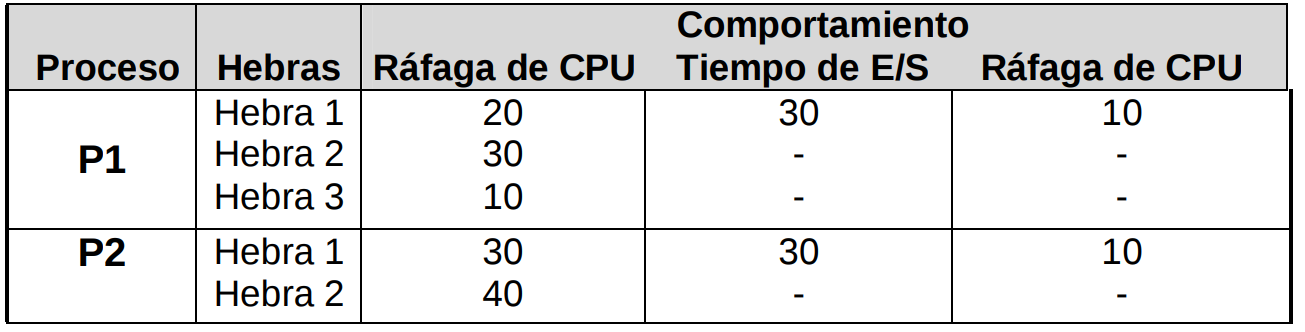
\includegraphics[scale=0.4]{images/tabla.png}
\end{figure}

\newpage

\begin{enumerate}[label=\alph*)]
	\item Para este apartado hay que tener en cuenta que en las hebras de usuario, el bloqueo de una implica el bloqueo del resto.
	
	\begin{figure}[h]
		\centering
		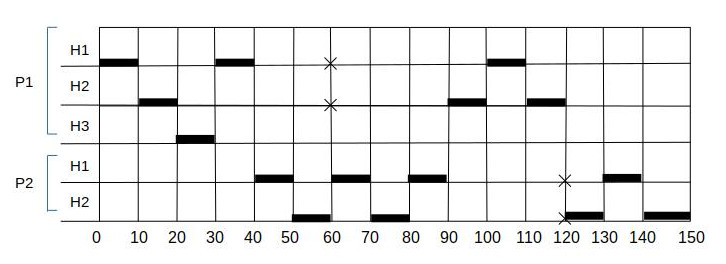
\includegraphics[scale=0.7]{images/apartadoA.jpg}
		\caption{Diagrama CPU apartado a)}
	\end{figure}
	
	Por tanto, el grado de ocupación vendrá dado por
	\[
	\left.
	\begin{array}{l}
	\text{Tiempo de CPU: } 150 \\
	\text{Tiempo total: } 150
	\end{array}
	\right\} \qquad \text{Grado de ocupación: } \frac{150}{150} = 1 \Rightarrow 100\%
	\]
	
	\bigskip
	
	\item En este caso, el núcleo sí distingue las hebras como tal y no las trata como el proceso global, por tanto no se debe de considerar quantum para el proceso global.
	
	\begin{figure}[h]
	\centering
	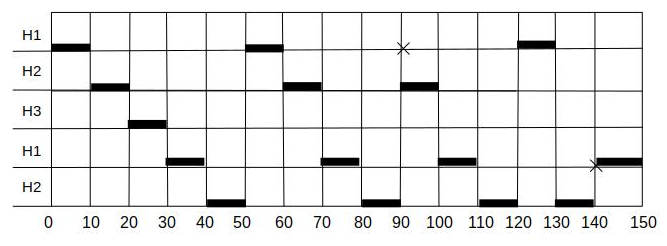
\includegraphics[scale=0.7]{images/apartadoB.jpg}
	\caption{Diagrama CPU apartado b)}
	\end{figure}
	
	Por tanto, el grado de ocupación vendrá dado por
	\[
	\left.
	\begin{array}{l}
	\text{Tiempo de CPU: } 150 \\
	\text{Tiempo total: } 150
	\end{array} 
	\right\} \qquad \text{Grado de ocupación: } \frac{150}{150} = 1 \Rightarrow 100\%
	\]
\end{enumerate}

La conclusión a la que llegamos es que en ambos modelos se presenta la misma eficiencia para este caso.
\end{document}
